\section{Experiments}
\label{sec:experiments}
In this section, we evaluate our method using  TU-Berlin sketch benchmark. It contains 250 classes. Each class has 80 instances. We do a group of experiments to compare our method with other methods in recognition speed and accuracy. Like previous works, we use 3-fold cross-validation within the dataset.


\subsection{Recognition accuracy with different $N$}
\label{ssec:resample_number}

From the Fig.~\ref{fig:resample}, we can see that 1024 points are enough to represent a tree. 512 points can also represent a tree but a little sparser. Even a tree with 256 points are visually clear for humans. In order find a proper $N$, we did a group experiments with $N = 1024, 512, 256, 128$. If $N$ is too large, there are no good for recognition accuracy, but makes recognition speed slower.

\begin{table}[htbp]
\begin{tabular}{|p{1.4cm}|p{1.3cm}|p{1.3cm}|p{1.3cm}|p{1.3cm}|}
    \hline
     $N$ & 1024& 512 & 256 & 128\\
    \hline
     accuracy & x\% & x\% & x\%& x\%\\
    \hline
     time & x & x & x& x\\
    \hline
\end{tabular}
\caption{Classification with different $N$.}
\end{table}

\subsection{Comparison of different methods in recognition speed and accuracy}
\label{ssec:cm_speed}
SketchPointNet is derived from PointNet. It uses lots of shared architecture, which means less parameters compared with existing Image-based sketch recognition approaches. We performed Sketch-a-Net(vallina), DeepSketch 1 and SketchPointNet on Titan 1080 with tensorflow 1.2. The whole model of Sketch-a-Net and DeepSketch 2 \cite{Dupont2016DeepSketch2D} use different feature fusion method, which makes the whole models too large to suite the mobile computing device. So we only compare 3 end-to-end networks(Sketch-a-Net(vallina), DeepSketch 1 and SketchPointNet).

\begin{table}[htbp]
\centering
\begin{tabular}{cccc}
    \hline
     -&Sketch-a-Net(vallina)& DeepSketch 1& Ours\\
    \hline
     model size& 64M&223M& 33M\\
     speed &10.9ms&10.6ms& 2.5ms\\
    \hline
\end{tabular}
\caption{Performance comparison of different networks.}
\label{tbl:speed}
\end{table}
From the tabel ~\ref{tbl:speed} we can see that our model is faster and smaller than Sketch-a-Net(vallina) and DeepSketch 1. Although our model are smaller compared with existing DNN-based appraches. We still achieve a high recognition accuracy.

\begin{table}[htbp]
\centering
\small
\begin{tabular}{lcc}
    \hline
     models &accuracy &end-to-end \\
    \hline
     HOG-SVM (Eitz et al, 2012)& 56\% &-\\
     Ensemble (Li et al, 2013) &61.5\% &-\\
     MKL-SVM (Li et al, 2015) & 65.8\% &-\\
     FV-SP (Schneider and Tuytelaars, 2014) & 68.9\% &-\\
     LeNet (LeCun et al, 2012)& 55.2\% &Yes\\
     Sketch-a-Net(vallina)(Yu et al, 2015)& 72.6\% &Yes\\
     Sketch-a-Net(Yu et al, 2016)& 77.95\% &No\\
     DeepSketch 1(Seddati et al, 2015)& 75.42\% &Yes\\
     DeepSketch 2(Seddati et al, 2016)& 77.69\% &No\\
     Our Model& 70.4\% &Yes\\
    \hline
\end{tabular}
\caption{Sketch recognition with different models.}
\label{tbl:acc}
\end{table}

Fig. ~\ref{fig:resshow} shows some results. Although our network can handle some challenging cases(green). SketchPointNet still fail on very ambiguous cases(the reds are predictions, the blacks are ground truth for each case).

\begin{figure}[htbp]
    \center
    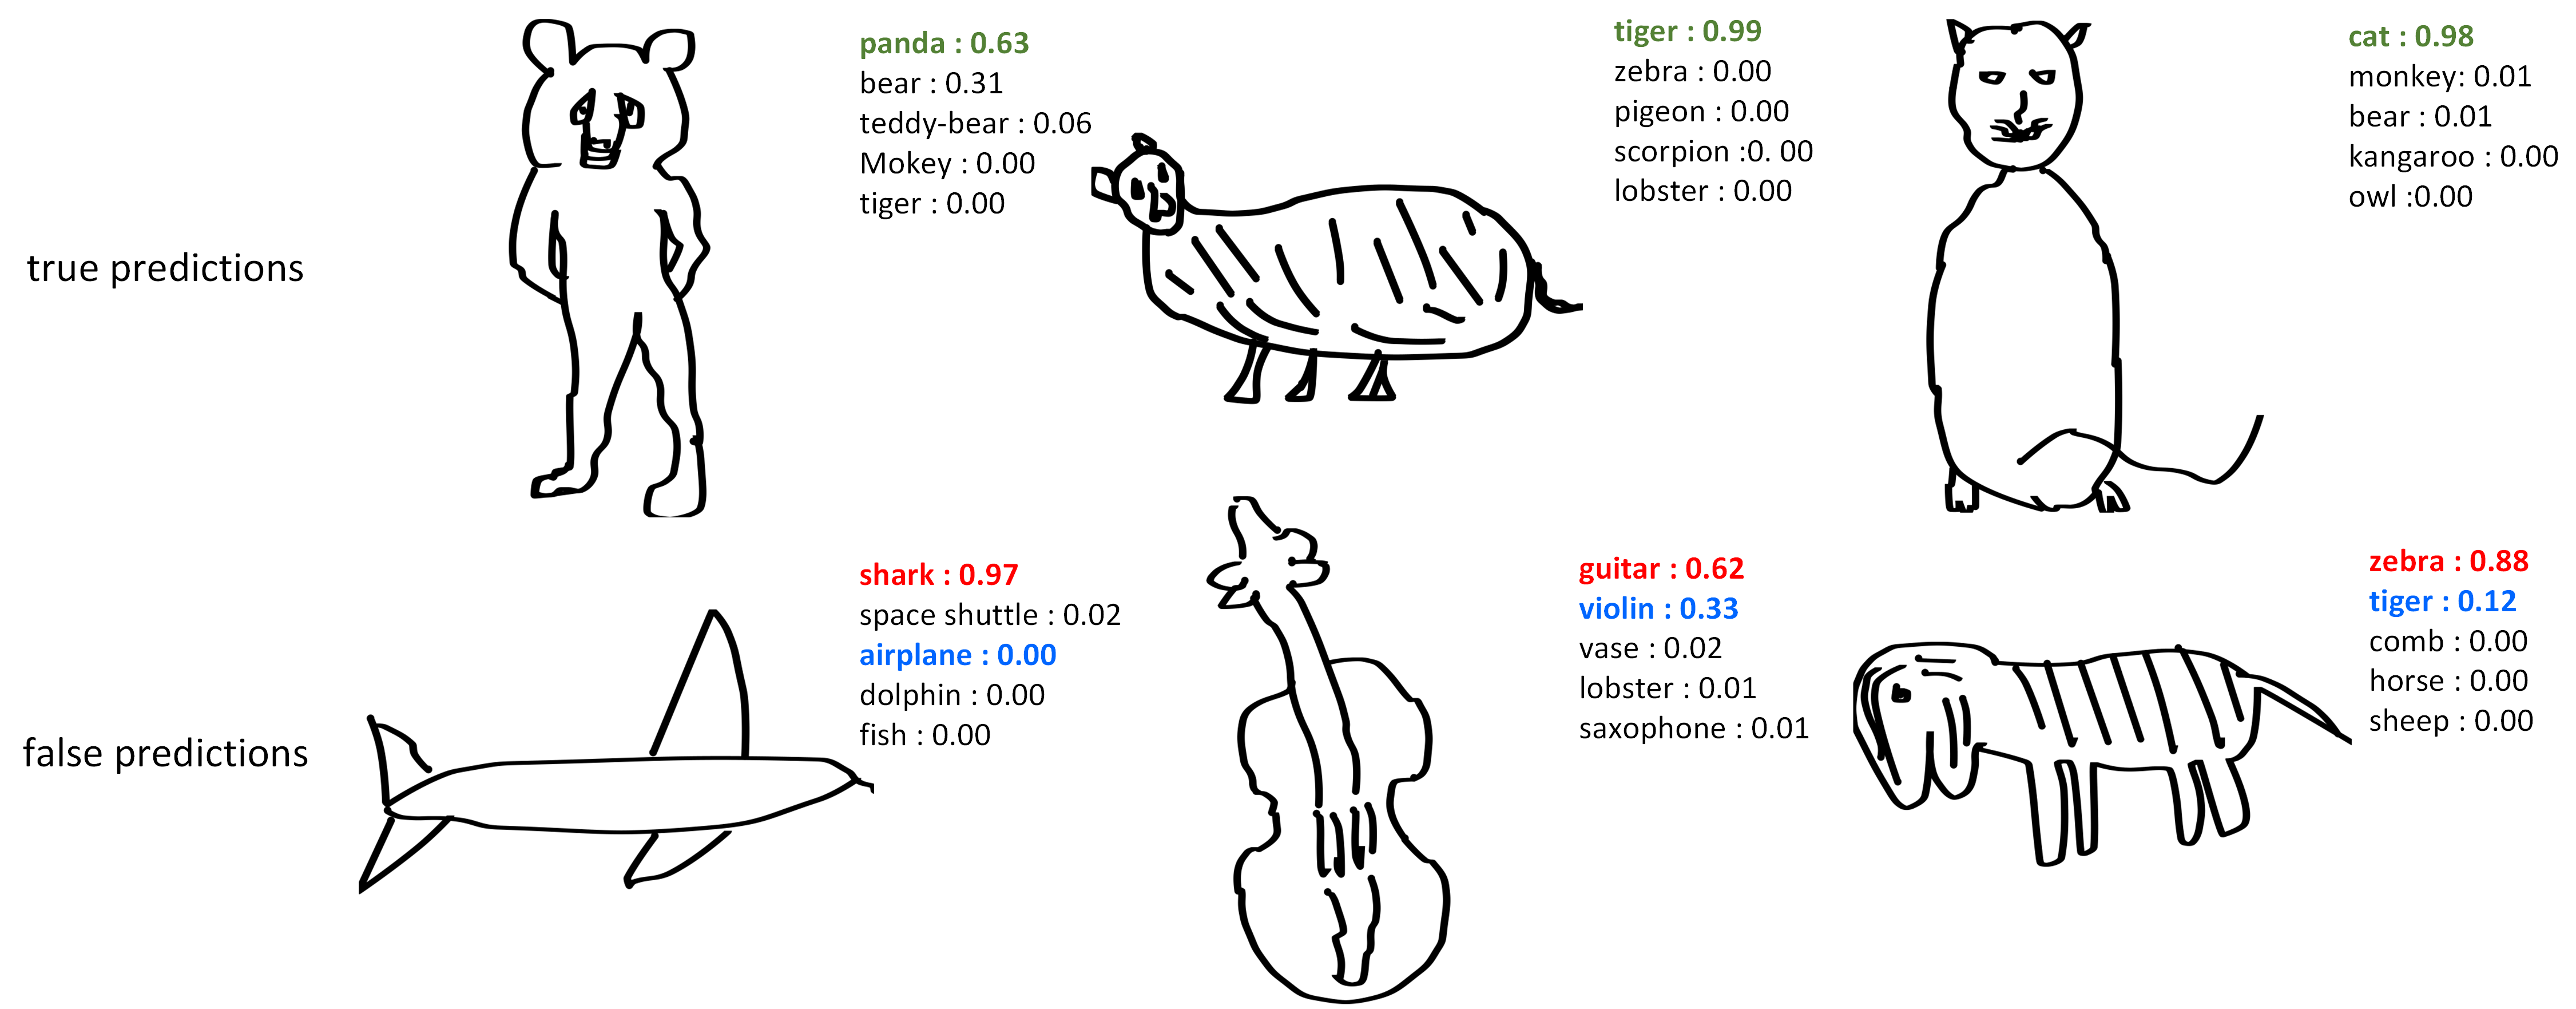
\includegraphics[width=3in]{images/res.png}
    \fcaption{Illustration of recognition successes (green) and failures (red).}
    \label{fig:resshow}
\end{figure}